\documentclass[10pt,a4paper]{article}
\usepackage[utf8]{inputenc}
\usepackage{amsmath}
\usepackage{amsthm}
\usepackage{amsfonts}
\usepackage{amssymb}
\usepackage{pgfplots}
\usepackage[english]{babel}
\usepackage{fourier}
\usepackage[left=2cm,right=2cm,top=2cm,bottom=2cm]{geometry}
\theoremstyle{definition}
\newtheorem{defn}{Definition}
\pgfplotsset{compat=1.9}
\newcommand*\Eval[3]{\left.#1\right\rvert_{#2}^{#3}}
\title{Algorithms Test 1 Review}
\author{Benjamin Boudra}
\begin{document}
\maketitle
\tableofcontents
\section{EX 1}
\subsection{Prompt}
\subsection{Answer}

\section{EX 2}
\subsection{Prompt}
\subsection{Answer}

\section{EX 3}
\subsection{Prompt}
Use the technique of bounding definite integrals to find the $\Theta$ category for the function.
\begin{equation}
  A (n) = log_2(1) + log_2(2) + log_2(3) + \ldots + log_2(n-1) + log_2(n)
\end{equation}
Actually, you should use the integral bound technique for one equality, and use trivial analysis for the other.
\subsection{Answer}
\subsubsection{Step 1: Draw a graph of the summation and Integral}
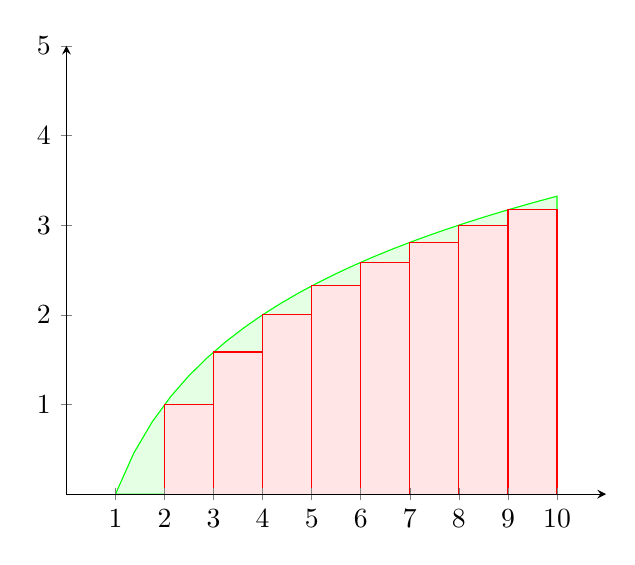
\begin{tikzpicture}
\begin{axis}[
    xtick={0,1,2,3,4,5,6,7,8,9,10},ytick={0,...,10},
    xmax=11,ymax=5,ymin=0,xmin=0,
    enlargelimits=true,
    axis lines=middle,
    clip=false,
    domain=0:11,
    axis on top
    ]

\addplot[draw=green, fill=green!10,domain=1:10]{ln(x)/ln(2)}\closedcycle;
\addplot [draw=red, fill=red!10, ybar interval, samples=10, domain=1:10]
    {ln(x)/ln(2)}\closedcycle;
\end{axis}
\end{tikzpicture}

\subsubsection{Step 2: Deduce the Graph's implications}
Following from the facts that:
\begin{enumerate}
  \item The integral is the area under the function $log_2(x)$ from $1$ to $n$.
  \item If we chose to view the integral as the summation of all of its length one segments from $1$ to $n$ plus the integral of whatever is left over (if n is not an integer value), the resulting integral's value will be unaffected.
  \item The value of each integral segment is greater than the value of its corresponding series segment because:
  \begin{enumerate}
    \item the value of the function and the series are equal at integer values
    \item the value of the function increases between integers and the value of the series does not.
  \end{enumerate}
\end{enumerate}
$\int_1^n log_2(x)$ is greater than $\sum_{i = 1}^n log_2(i)$ for any $n$ greater than $1$. Thus, to find the upper bound or $O$ of $\sum_{i = 1}^n log_2(i)$ we merely need to find the integral of $\int_1^n log_2(x)$\\\\
\subsubsection{Step 3: Calculate the Definite integral}
So now I will calculate $\int_1^n log_2(x)$
\begin{enumerate}
  \item Recognize that to take the integral of a logarithm, we will have to perform integration by parts. so we must chose $u$ and $dv$ values.
  \begin{equation}
    u = log_2(x)\qquad du = 1/xln(2) \qquad dv = 1 \qquad v = x
  \end{equation}
  \item solve for the indefinite integral
  \begin{multline}
    \int_1^n log_2(x) = \Eval{\frac{ln(x)*x}{ln(2)}}{1}{n}- \int_1^n \frac{x}{xln(2)} = \Eval{\frac{ln(x)*x}{ln(2))}}{1}{n} - \int_1^n \frac{1}{ln(2)} = \Eval{\frac{ln(x)*x}{ln(2)} - \frac{x}{ln(2)}}{1}{n} = \\ \Eval{\frac{ln(x)*x-x}{ln(2)}}{1}{n}
  \end{multline}
  \item solve for the definite integral
  \begin{equation*}
    \Eval{\frac{ln(x)*x-x}{ln(2)}}{1}{n} = \frac{ln(n)*n-n}{ln(2)} - \left(\frac{ln(1)*1-1}{ln(2)}\right) = \frac{ln(n)*n-n}{ln(2)} + \left(\frac{1}{ln(2)}\right) = \frac{ln(n)*n-n + 1}{ln(2)}
  \end{equation*}
\end{enumerate}
Thus, The equation:
\begin{equation*}
  \frac{ln(n)*n-n + 1}{ln(2)}
\end{equation*}
Acts as an upper bound for the summation.
\subsubsection{Step 4: Prove Upper Bound is in $\Theta(n log(n))$}
According to our notes, an equation has the time complexity category of $\Theta(n)$ if it satisfies the following definition:
  \begin{defn}
    For functions $f$ and $g$, we can say that $f \in \Theta(g) \iff $ there is a positive integers $N,M$ and positive real numbers $n,m$ such that the following equations are satisfied:
    \begin{equation*}
      \forall_{ n > N}, f(n) \leq cg(n) \qquad \text{also known as O(n)}
    \end{equation*}
    and
    \begin{equation*}
      \forall_{ m > M}, f(m) \geq cg(m) \qquad \text{also known as }\Omega\text{ (n)}
    \end{equation*}
  \end{defn}
\begin{enumerate}
  \item prove equation is $O(n log(n))$.\\
  \begin{enumerate}
    \item chose $c$ value, $c = 1/ln(2)$
    \item solve for $n$.
    \begin{equation*}
      \frac{ln(n)*n-n+1}{ln(2)} \leq \frac{n*ln(n)}{ln(2)}
    \end{equation*}
    \begin{multline*}
      0 \leq \frac{n*ln(n)}{ln(2)} - \frac{ln(n)*n-n+1}{ln(2)} = 0 \leq \frac{n*ln(n)}{ln(2)} - \frac{ln(n)*n-n+1}{ln(2)} \\ = 0 \leq \frac{n*ln(n) - n*ln(n)+n-1}{ln(2)}= 0  \leq \frac{n-1}{ln(2)} =  1 \leq n
    \end{multline*}
    \item Thus we shall chose n = 1 and we have proven:
    \begin{equation*}
       \frac{ln(n)*n-n+1}{ln(2)} \in O(nln(n))
    \end{equation*}
  \end{enumerate}
  \item Prove equation is $\Omega(n log(n))$.
  \begin{enumerate}
    \item chose $c$ value, $c = \frac{1}{2ln(2)}$
    \item solve for $n$
    \begin{equation*}
      \frac{ln(n)*n-n+1}{ln(2)} \geq \frac{n*ln(n)}{2ln(2)}
    \end{equation*}
    \begin{multline*}
      0 \geq \frac{n*ln(n)}{2ln(2)} - \frac{ln(n)*n-n+1}{ln(2)} = 0 \geq \frac{n*ln(n)}{ln(2)} - \frac{2*(ln(n)*n-n+1)}{ln(2)} = 0 \geq \frac{n*ln(n)-2ln(n)*n+2n-2}{ln(2)} \\ = 0 \geq \frac{-ln(n)*n+2n-2}{ln(2)}
    \end{multline*}
    Use calculator to solve for $n$ in equation and you get:
    \begin{equation*}
      n \geq 1
    \end{equation*}
    Thus we shall choose n=1 and the equation is true, thus we have proven:
    \begin{equation}
       \frac{ln(n)*n-n+1}{ln(2)} \in \Omega(nln(n))
    \end{equation}
    \item Prove equation is in $\Theta(n*log(n))$.

    According to definition 1 above: A function is in $\Theta(nlog(n))$ if it has a $O(nlog(n))$ and a $\Omega(n*log(n)$. We have proven that it has both. Therefore the function:
    \begin{equation*}
       \frac{ln(n)*n-n+1}{ln(2)} \in \Theta(nln(n))
    \end{equation*}
  \end{enumerate}
\end{enumerate}
\subsubsection{Step 5: Find Lower Bound}
If we shift the original function $log_2(x)$ over one position to the right by adding 1 to the $x$ coordinate to get the function $log_2(x-1)$. The summation function $\sum_1^n ln(n)$ will be larger than $\int_1^n ln(n)$ because if we break up the integral into a sum of smaller integrals like we did in step 2, each summation segment will be larger than its corresponding integral segment for the following reasons:
\begin{itemize}
  \item At the beginning of each integer, the integral segment's value is smaller than the series equivalent.
  \item Between integers the value of the integral segment will approach the value of the summation segment. However, it will never pass it.
  \item Due to the fact that the function is always increasing in size. This pattern will continue infinitely.
\end{itemize}
See the graph below for a visual reference:

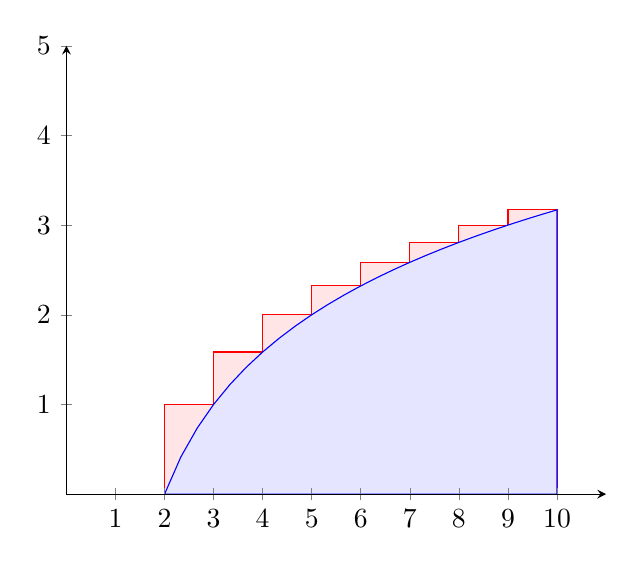
\begin{tikzpicture}
\begin{axis}[
    xtick={0,1,2,3,4,5,6,7,8,9,10},ytick={0,...,10},
    xmax=11,ymax=5,ymin=0,xmin=0,
    enlargelimits=true,
    axis lines=middle,
    clip=false,
    domain=0:11,
    axis on top
    ]
\addplot [draw=red, fill=red!10, ybar interval, samples=10, domain=1:10]
    {ln(x)/ln(2)}\closedcycle;
\addplot[draw=blue, fill=blue!10,domain=2:10]{ln(x-1)/ln(2)}\closedcycle;
\end{axis}
\end{tikzpicture}

\subsubsection{Find Integral of $log_2(x-1)$}
For simplicity:
\begin{equation*}
  log_2(x-1) = \frac{ln(x-1)}{ln(2)}
\end{equation*}

\begin{enumerate}
  \item Choose u and dv
  \begin{equation}
    u = \frac{ln(x-1)}{ln(2)} \qquad du = ln
  \end{equation}
\end{enumerate}
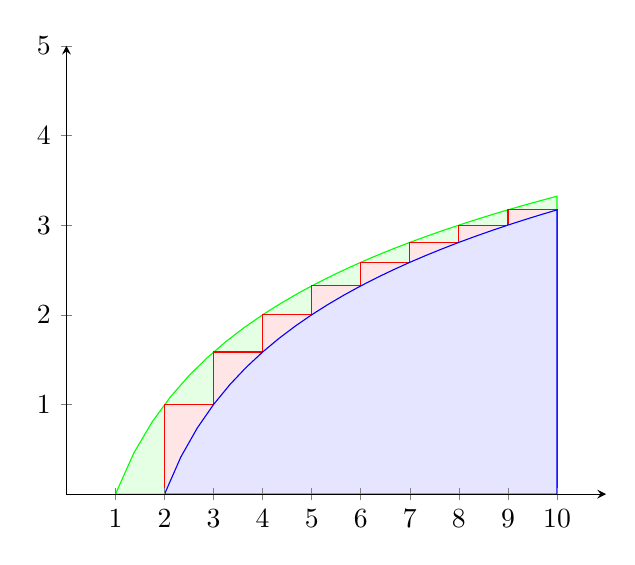
\begin{tikzpicture}
\begin{axis}[
    xtick={0,1,2,3,4,5,6,7,8,9,10},ytick={0,...,10},
    xmax=11,ymax=5,ymin=0,xmin=0,
    enlargelimits=true,
    axis lines=middle,
    clip=false,
    domain=0:11,
    axis on top
    ]
\addplot[draw=green, fill=green!10,domain=1:10]{ln(x)/ln(2)}\closedcycle;
\addplot [draw=red, fill=red!10, ybar interval, samples=10, domain=1:10]
    {ln(x)/ln(2)}\closedcycle;
\addplot[draw=blue, fill=blue!10,domain=2:10]{ln(x-1)/ln(2)}\closedcycle;
\end{axis}
\end{tikzpicture}
\section{EX 4}
\subsection{Prompt}
\subsection{Answer}

\section{EX 5}
\subsection{Prompt}
\subsection{Answer}

\section{EX 6}
\subsection{Prompt}
\subsection{Answer}

\section{EX 7}
\subsection{Prompt}
\subsection{Answer}

\end{document}
